% ============ §6 数值验证与灵敏度 ============
\section{数值验证与灵敏度分析}

\subsection{多层次数值验证}

本文对数值结果做了三类验证，其结论已在各节给出，此处汇总。

\textbf{（1）解析与制造解验证。} 温度场：谱配点解与 5.1.2 解析解偏差
$1.6\times10^{-4}$\,°C；常扩散系数情形与 Bessel 级数解偏差
$9.5\times10^{-9}$。水分场（非线性）：构造光滑制造解并反推解析强迫项
\cite{roache}，谱解与制造解偏差 $6.1\times10^{-9}$；时间容差从 $10^{-8}$
收紧到 $10^{-12}$ 时误差由 $2.7\times10^{-7}$ 降至 $2.1\times10^{-10}$
（图~\ref{fig:mms}），表明误差受容差控制而非格式缺陷。

\begin{figure}[H]
\centering
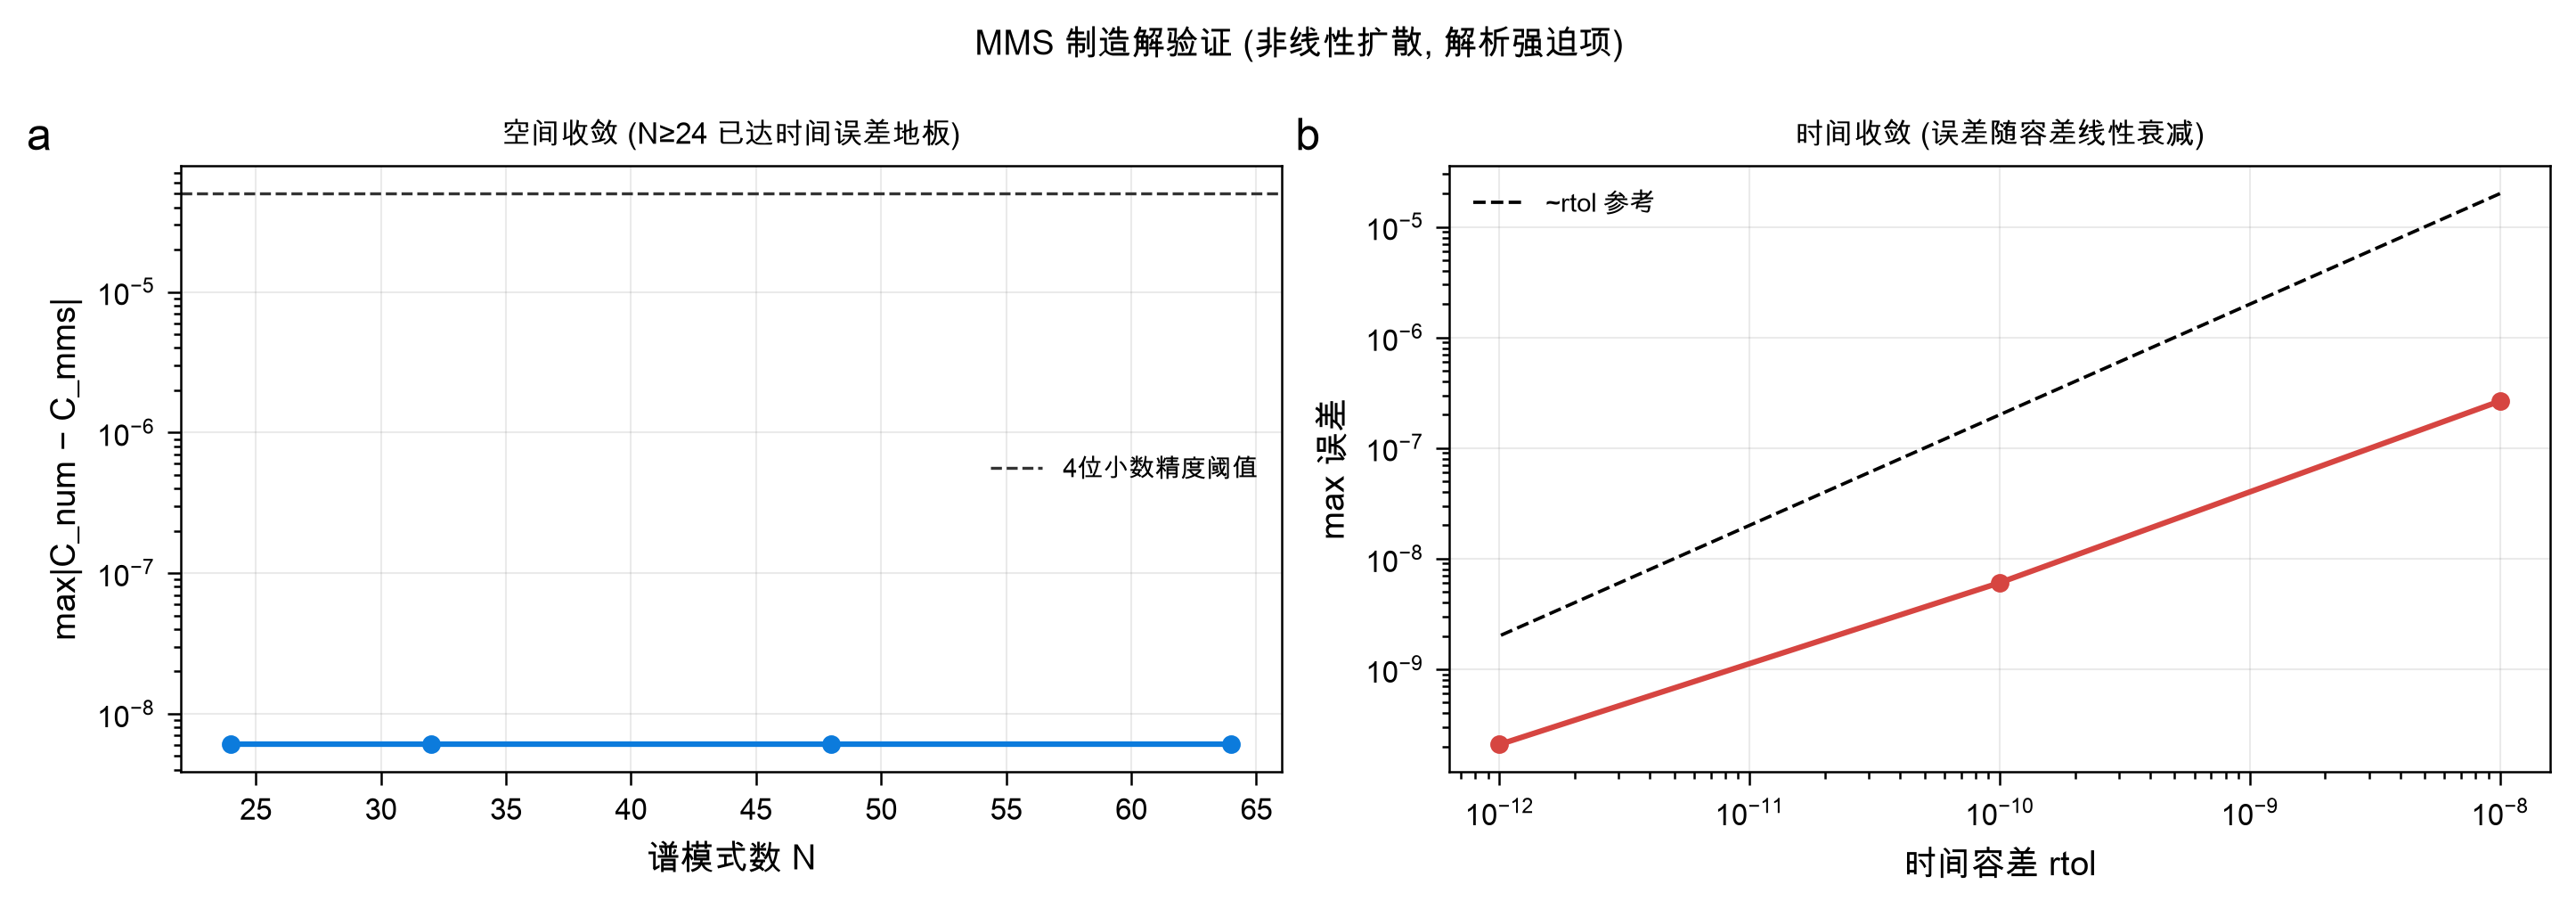
\includegraphics[width=0.95\textwidth]{fig7_mms.png}
\caption{制造解验证。（a）空间：$N\ge24$ 后谱误差低于时间误差水平；
（b）时间：误差随容差线性衰减。}
\label{fig:mms}
\end{figure}

\textbf{（2）空间与时间收敛。} 问题二给出了谱模式数 $N=48/96/128$ 的
收敛序列（表~\ref{tab:conv}），提交结果取 $N=128$；问题一末位谱系数
$5\times10^{-13}$。时间方向由 BDF 自适应控制（相对容差 $10^{-8}\sim10^{-9}$），
制造解验证确认误差随容差衰减。

\textbf{（3）独立算法交叉验证。} 全部四个问题均与独立实现的有限体积法
求解器交叉对比：问题一至三轨迹偏差 $6\times10^{-4}$ 以内、表 1--表 4
逐项 4 位小数一致；问题四与另一套坐标变换的离散结果偏差 0.02 h。两种
离散建立在不同坐标系与不同差分结构上，结果一致显著降低了由单一数值格式
或程序实现造成系统性错误的可能性（交叉验证不能替代对模型假设本身的检验，
后者见 7.2 节局限讨论）。

此外，谱配点法的边界条件在每次右端求值中由边界方程直接解出（残差
$10^{-19}$ 量级），问题四的随体网格满足几何守恒恒等式；Duhamel 解在
$\tau\to0$ 时退化为阶跃边界响应。这些内容在附录 B 中说明。

\subsection{灵敏度分析}

对五个关键参数做 OAT 单参数 $\pm10\%$ 扰动，输出指标为烘干时长
（表~\ref{tab:sens}，图~\ref{fig:tornado}）。

\begin{table}[H]
\centering
\caption{OAT 灵敏度（$\pm10\%$，QoI = 烘干时长）}
\label{tab:sens}
\begin{tabular}{ccccc}
\toprule
参数 & 名义值 & $\Delta t_{end}(-10\%)$ & $\Delta t_{end}(+10\%)$ & $|\Delta|$ 之和 \\
\midrule
$T_{bar}$（恒温段温度） & $49.969$\,°C & \textbf{+10.87 h} & \textbf{$-$8.68 h} & 19.55 h \\
$D$ 前置因子 & $2.4\times10^{-3}$ & +5.98 h & $-$4.90 h & 10.88 h \\
$\beta$（对流传质系数） & $8\times10^{-7}$ & +0.53 h & $-$0.45 h & 0.98 h \\
$h$（对流换热系数） & 25.0 & $-$0.02 h & $-$0.03 h & 0.05 h \\
\bottomrule
\end{tabular}
\end{table}

\begin{figure}[H]
\centering
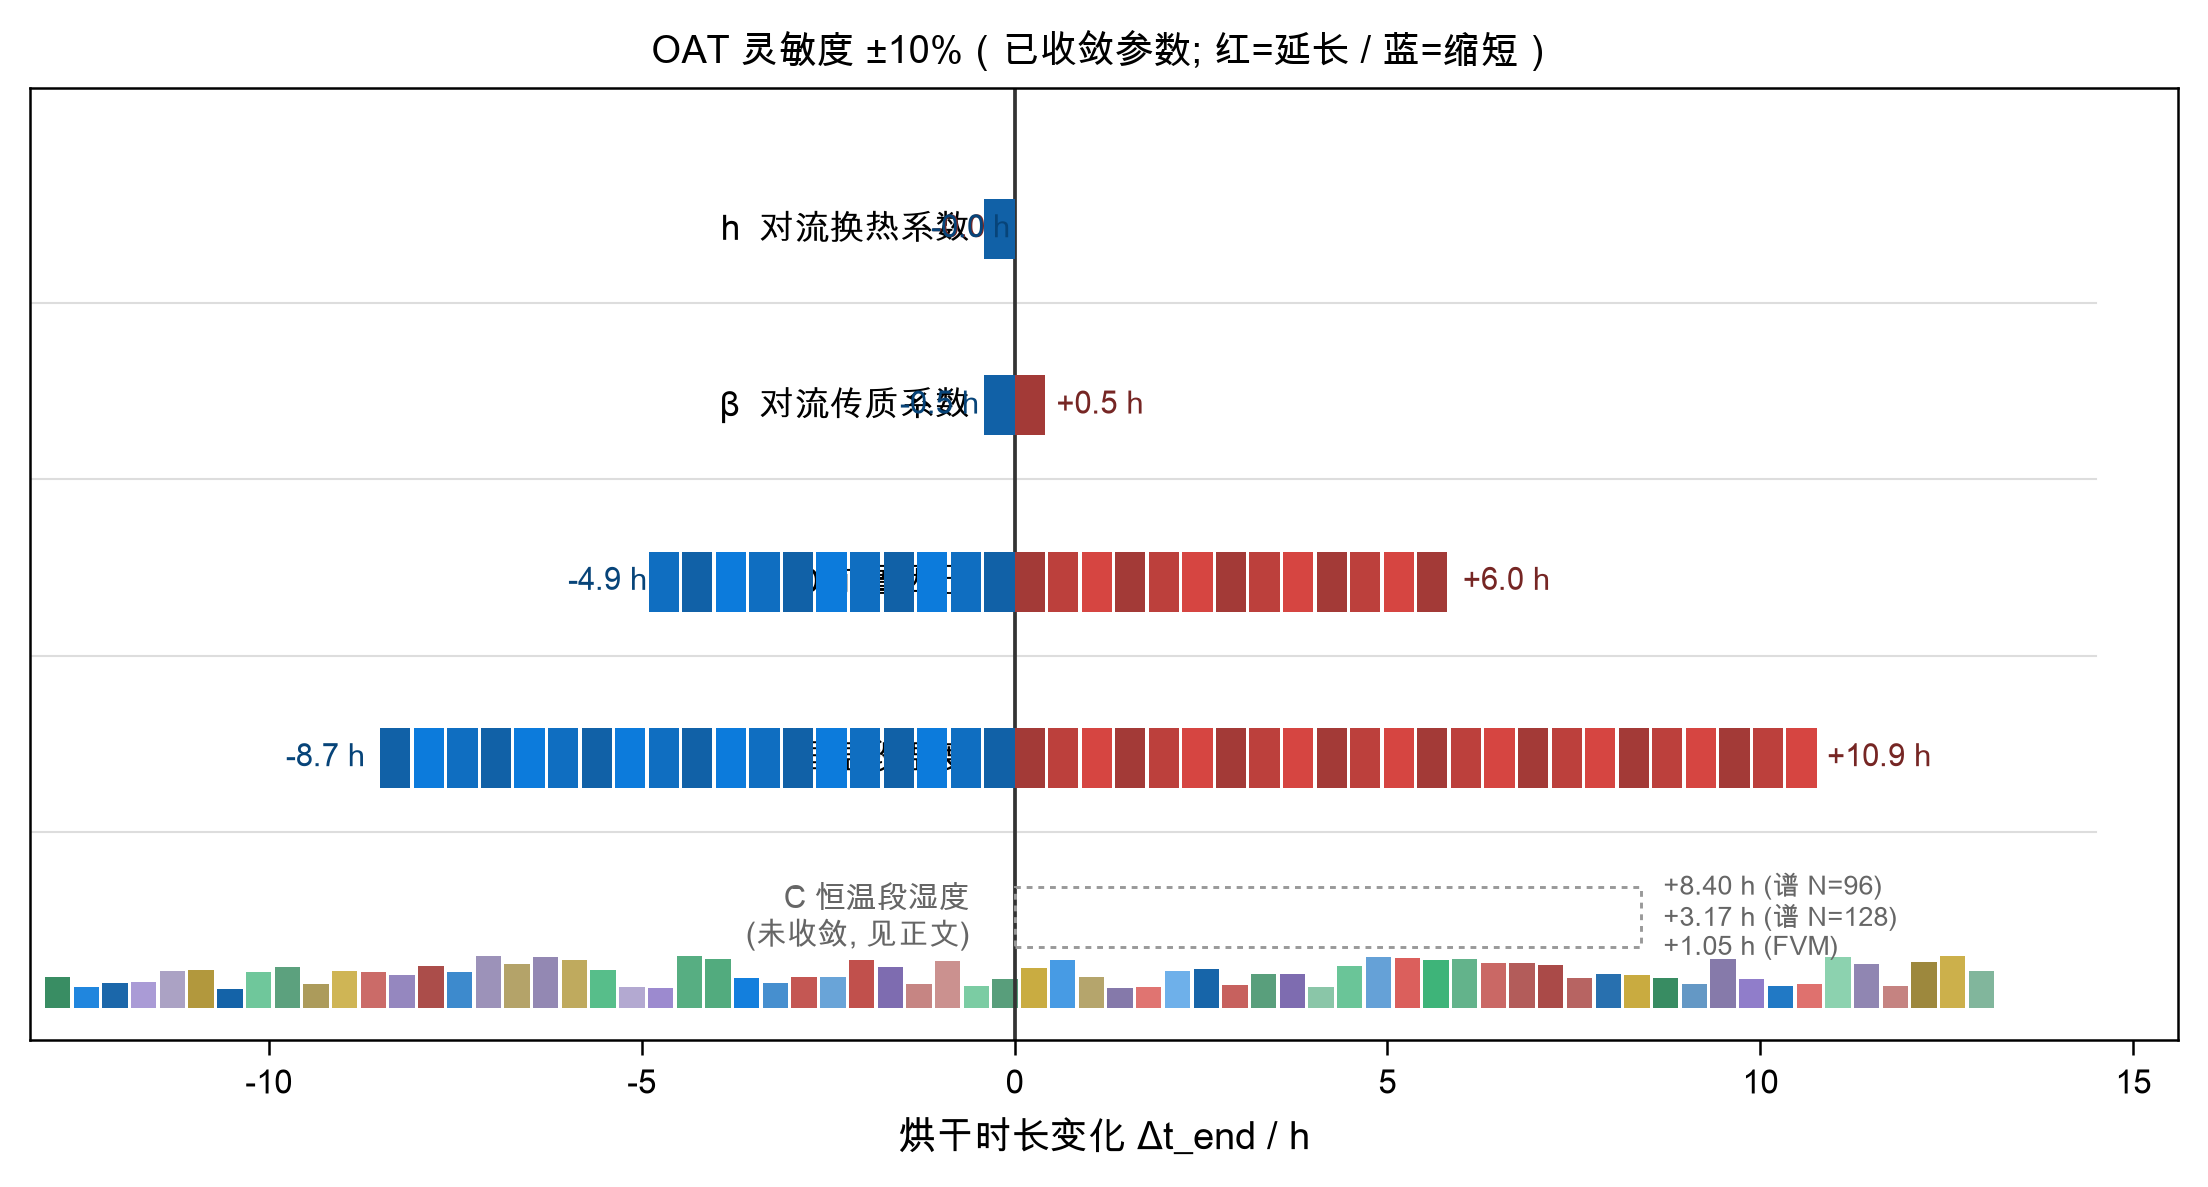
\includegraphics[width=0.72\textwidth]{fig10_tornado.png}
\caption{灵敏度 tornado 图。恒温段温度为主导控制量，换热系数影响可忽略。}
\label{fig:tornado}
\end{figure}

\textbf{解释。}\textbf{（1）温度的主导作用：}$T_{bar}$ 经 Arrhenius 项 $e^{-3850/T}$ 放大，
降温侧比升温侧更敏感（指数函数凸性所致）；\textbf{（2）传热非瓶颈：}$h$ 的影响
不足 \textbf{0.1 h}：热平衡在小时尺度内即可建立，而干燥持续数天，烘干时长由
水分扩散控制。上述四个参数两套方法给出的数值接近（有限体积法：
$T_{bar}$ $+10.40/-8.30$、$D$ 前置 $+5.73/-4.68$、$\beta$ $+0.68/-0.55$、
$h$ $\pm0.02$，单位 h），排序 $T_{bar}\gg D_{pre}>\beta>h$ 在两种方法中
一致。

\subsubsection{未收敛敏感项：恒温段湿度 $C_{bar}$}

$C_{bar}$ 的 $\pm10\%$ 扰动对空间分辨率敏感，随分辨率加密呈现单调
收敛趋势：

\begin{table}[H]
\centering
\caption{$C_{bar}-10\%$ 工况的烘干时长变化（分辨率收敛序列）}
\label{tab:cbar}
\begin{tabular}{lcc}
\toprule
方法 & 分辨率 & $\Delta t_{end}$ \\
\midrule
谱配点 & $N=96$ & $+8.40$ h \\
谱配点 & $N=128$ & $+3.17$ h \\
有限体积法 & 400 节点 & $+1.05$ h \\
\bottomrule
\end{tabular}
\end{table}

方向在全部分辨率下一致（$C_{bar}$ 降低延长干燥），幅度随分辨率加密由
8.4 h 收敛至 1--3 h 量级，但两种独立方法尚未完全一致。该工况的干燥锋面
更陡、对空间分辨率更敏感。本文将 $C_{bar}$ 单独列为未收敛敏感项，
不纳入主灵敏度排序；其定性方向（降湿延长干燥）成立，定量幅度以
1--3 h 量级估计。

% ============ §7 模型评价与推广 ============
\section{模型评价与推广}

\subsection{模型优点}

\begin{enumerate}
\item 问题一的温度场采用解析方法求解：该解在 $\tau\to0$ 时退化为阶跃
边界响应、在 $t=0$ 时恢复初值，两个极限情形均与已知解一致，并作为数值
求解器的独立基准；
\item 谱配点离散对光滑剖面指数收敛，配合末位谱系数误差指示，空间分辨率
不足时（问题二的干燥锋面）能够被直接发现并加密；
\item 问题四的随体坐标推导建立在干基含水率的物质守恒上，收缩边界处理
经另一套坐标变换独立验证；
\item 全部结果经过解析/制造解、收敛序列与独立算法三类交叉验证。
\end{enumerate}

\subsection{模型局限}

\begin{enumerate}
\item 谱方法对干燥锋面需要 $N\ge96$ 个模式（$N=48$ 时 $t_{end}$ 偏差约
14 h），二维推广时计算量增长较快；
\item 表面边界方程的求解依赖上一时刻表面值的延续，若环境条件出现阶跃式
突变需要重新论证解的连续性；
\item 问题四假设径向仿射收缩，题目仅提供径向数据，轴向与各向异性收缩
未建模；
\item 环境外推基于 0--4 h 数据，若恒温段存在更晚的工况变化，烘干时长的
偏移量以灵敏度分析（$T_{bar}$ $\pm10\%$ 对应 $-8.7\sim+10.9$ h）估计；
\item 题目参数体系未提供汽化潜热与局部相变速率，本文采用显热传导模型以
保持参数闭合，蒸发吸热对表面温度的修正未计入。
\end{enumerate}

\subsection{模型推广}

谱配点离散与随体坐标边界处理可直接推广至：片状/球状药材干燥（更换几何
因子）、果蔬脱水与粮食仓储干燥（同型有效扩散模型）、干燥工艺参数优化
（以恒温段温度为主导控制量的结论指导节能策略）。时间尺度比 $\Gamma$
的时空分布可用于干燥过程的阶段识别与工艺控制设计。
